\chapter{Digital CMS pixel chip}

The digital CMS pixel chip, colloquially called \glsreset{ROC}\gls{ROC}, consists of 52$\times$80~pixels. Electrically they are organized in 26 double columns, each having 2$\times$80~pixels. One double column is controlled by a periphery which has buffers for time-stamps and data. There are 24~time-stamp buffers (8~bit wide) and 80~data buffers, see Fig.~\ref{UNDEFINED}

\begin{figure}[hbtp]
    \begin{center}
	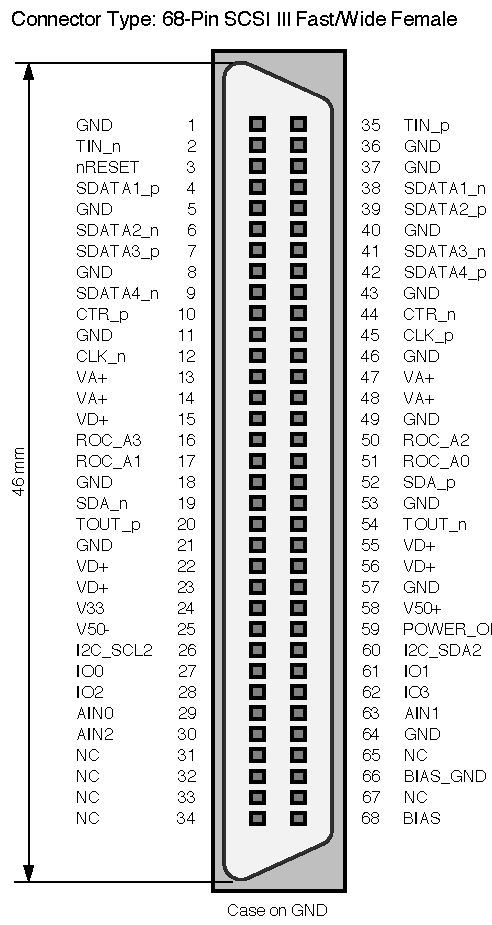
\includegraphics[width=85mm]{img/DTB_adapterplug.pdf}
	\caption{ROC/Module interface connector pin scheme.}
	\label{fig:ROCmoduleInterfaceConnector}
    \end{center}
\end{figure}

\begin{table}[h]
    \begin{center}
	\caption{\textbf{DAC and registers.} The values being sent to the ROC are 4 or 8 bit words.}
	\label{tab:DecBinHex}

	\bigskip

	{\scriptsize
	\begin{tabular}{lrccrrrl}
	\toprule
	Name & addr & unit & \# bits & \multicolumn{1}{p{0.8cm}}{Min Value} & \multicolumn{1}{p{0.8cm}}{Max Value} & \multicolumn{1}{p{1.2cm}}{Recomm. DAC Value} & Description \\ 
	\midrule
	\multicolumn{ 8}{l}{\textbf{Voltage Regulators}} \\ 
	Vdd         &  1 &   mV    & 4 & 1700 & 2100 & 6 & Voltage regulator for digital supply \\ 
	Vana        &  2 &   mA    & 8 & 5 & 65 & 90 & Current regulator for analog supply \\ 
	Vsh         &  3 &   mA    & 8 & 1 & 14 & 40 & Current regulator for sample \& hold circuit \\ 
	Vcomp       &  4 &   mV    & 4 & 1800 & 2100 & 12 & Voltage regulator for comparator \\ 
	\midrule
	\multicolumn{ 8}{l}{\textbf{Analog PUC}} \\ 
	VwllPr      &  7 &   mV    & 8 & 400 & 1300 & 60 & Preamplifier feedback  \\ 
	VwllSh      &  9 &   mV    & 8 & 400 & 1300 & 60 & Shaper feedback \\ 
	VHldDel     & 10 &   mV    & 8 & -1500 & -500 & 117 & Hold delay \\ 
	Vtrim       & 11 &   mV    & 8 & -710 & -400 & 29 & Pixel trimming \\ 
	VcThr       & 12 &   mV    & 8 & -1500 & -600 & 60 & Comparator threshold \\ 
	\midrule
	\multicolumn{ 8}{l}{\textbf{Pixel Readout}} \\ 
	VIbias\_bus & 13 & $\mu$A  & 8 & 0 & 12 & 5 & Digital bus receiver \\ 
	VIbias\_sf  & 14 & $\mu$A  & 4 & 0 & 50 & 6 & Analog bus receiver \\ 
	VIColOr     & 22 & $\mu$A  & 8 & 0 & 200 & 20 & Current limiter \\ 
	\midrule
	\multicolumn{ 8}{l}{\textbf{Double Column Readout}} \\ 
	VOffsetOp   & 15 &   mV    & 8 & 1000 & 1500 & 90 & Charge amplifier offset \\ 
	VOffsetRO   & 17 &   mV    & 8 & 1000 & 1500 & 76 & Voltage amplifier offset \\ 
	VIon        & 18 & $\mu$A  & 8 & 0 & 100 & 115 & Voltage amplifier bias current \\ 
	\midrule
	\multicolumn{ 8}{l}{\textbf{Chip Readout}} \\ 
	Vcomp\_ADC  & 19 & mV & 8  & 600 & 1050 & 100 & ADC comparator voltage \\ 
	VIref\_ADC  & 20 & $\mu$A  & 8 & 0 & 12 & 160 & ADC reference current \\ 
	\midrule
	\multicolumn{ 8}{l}{\textbf{Others}} \\ 
	Vcal        & 25 & mV      & 8 & 0 & 260/1800 & 150 & Calibrate pulse height, see also section 5.3.5 \\ 
	CalDel      & 26 & nsec    & 8 & 55 & 205 &  & See chapter 7 \\ 
	WBC         & 254 & clocks & 8 & 0 & 255 &                 >70 & Trigger latency \\ 
	CCR         & 253 &        & 8 &  &  &  & See section 5.3.5 \\ 
	\bottomrule
	\end{tabular}
	}
    \end{center}
\end{table}


